\documentclass[answers]{exam}
\newif\ifanswers
\answerstrue % comment out to hide answers

\usepackage{lastpage} % Required to determine the last page for the footer
\usepackage{extramarks} % Required for headers and footers
\usepackage[usenames,dvipsnames]{color} % Required for custom colors
\usepackage{graphicx} % Required to insert images
\usepackage{listings} % Required for insertion of code
\usepackage{courier} % Required for the courier font
\usepackage{lipsum} % Used for inserting dummy 'Lorem ipsum' text into the template
\usepackage{enumerate}
\usepackage{subfigure}
\usepackage{booktabs}
\usepackage{amsmath, amsthm, amssymb}
\usepackage{hyperref}
\usepackage{datetime}
\usepackage{minted}
\settimeformat{ampmtime}
\usepackage{algpseudocode}
\usepackage{algorithmicx}
\usepackage[ruled]{algorithm}
\usepackage{tikz-dependency}

\usepackage{tikz}
\usepackage{amsfonts}
\usetikzlibrary{positioning,patterns,fit,calc}
% Margins
\topmargin=-0.45in
\evensidemargin=0in
\oddsidemargin=0in
\textwidth=6.5in
\textheight=9.0in
\headsep=0.25in

\linespread{1.1} % Line spacing

% Set up the header and footer
%\pagestyle{fancy}
%\rhead{\hmwkAuthorName} % Top left header
%\lhead{\hmwkClass: \hmwkTitle} % Top center head
%\lfoot{\lastxmark} % Bottom left footer
%\cfoot{} % Bottom center footer
%\rfoot{Page\ \thepage\ of\ \protect\pageref{LastPage}} % Bottom right footer
%\renewcommand\headrulewidth{0.4pt} % Size of the header rule
%\renewcommand\footrulewidth{0.4pt} % Size of the footer rule

\pagestyle{headandfoot}
\runningheadrule{}
\firstpageheader{CS 224n}{Assignment 3}{}
\runningheader{CS 224n} {Assignment 3} {Page \thepage\ of \numpages}
\firstpagefooter{}{}{} \runningfooter{}{}{}

\setlength\parindent{0pt} % Removes all indentation from paragraphs

%----------------------------------------------------------------------------------------
%	CODE INCLUSION CONFIGURATION
%----------------------------------------------------------------------------------------

\definecolor{MyDarkGreen}{rgb}{0.0,0.4,0.0} % This is the color used for comments
\lstloadlanguages{Python} % Load Perl syntax for listings, for a list of other languages supported see: ftp://ftp.tex.ac.uk/tex-archive/macros/latex/contrib/listings/listings.pdf
\lstset{language=Python, % Use Perl in this example
    frame=single, % Single frame around code
    basicstyle=\footnotesize\ttfamily, % Use small true type font
    keywordstyle=[1]\color{Blue}\bf, % Perl functions bold and blue
    keywordstyle=[2]\color{Purple}, % Perl function arguments purple
    keywordstyle=[3]\color{Blue}\underbar, % Custom functions underlined and blue
    identifierstyle=, % Nothing special about identifiers
    commentstyle=\usefont{T1}{pcr}{m}{sl}\color{MyDarkGreen}\small, % Comments small dark green courier font
    stringstyle=\color{Purple}, % Strings are purple
    showstringspaces=false, % Don't put marks in string spaces
    tabsize=5, % 5 spaces per tab
%
% Put standard Perl functions not included in the default language here
    morekeywords={rand},
%
% Put Perl function parameters here
    morekeywords=[2]{on, off, interp},
%
% Put user defined functions here
    morekeywords=[3]{test},
%
    morecomment=[l][\color{Blue}]{...}, % Line continuation (...) like blue comment
    numbers=left, % Line numbers on left
    firstnumber=1, % Line numbers start with line 1
    numberstyle=\tiny\color{Blue}, % Line numbers are blue and small
    stepnumber=5 % Line numbers go in steps of 5
}

%----------------------------------------------------------------------------------------
%	NAME AND CLASS SECTION
%----------------------------------------------------------------------------------------

\newcommand{\hmwkTitle}{Dependency Parsing} % Assignment title
\newcommand{\hmwkClass}{CS\ 224n Assignment \#3} % Course/class
\newcommand{\ifans}[1]{\ifanswers \color{red} \textbf{Solution: } #1 \color{black} \fi}

\input macros.tex
\input std_macros.tex

%----------------------------------------------------------------------------------------
%	TITLE PAGE
%----------------------------------------------------------------------------------------
\qformat{\Large\bfseries\thequestion{}. \thequestiontitle{} (\thepoints{})\hfill}

\title{
    \vspace{-1in}
    \textmd{\textbf{\hmwkClass:\ \hmwkTitle} \\ \hmwkAuthorName}\\
}
\author{}
%\date{\textit{\small Updated \today\ at \currenttime}} % Insert date here if you want it to appear below your name
\date{}

\setcounter{section}{0} % one-indexing
\begin{document}

    \maketitle

    \begin{center}
        \large{\textbf{Due on} Tuesday Jan. 25, 2022 by \textbf{3:15pm (before class)}}
    \end{center}

    In this assignment, you will build a neural dependency parser using PyTorch. For a review of the fundamentals of PyTorch, please check out the PyTorch review session on Canvas. In Part 1, you will learn about two general neural network techniques (Adam Optimization and Dropout). In Part 2, you will implement and train a dependency parser using the techniques from Part 1, before analyzing a few erroneous dependency parses.
    \begin{questions}
        \graphicspath{ {images/} }

% real numbers R symbol
\newcommand{\Real}{\mathbb{R}}

% encoder hidden
\newcommand{\henc}{\bh^{\text{enc}}}
\newcommand{\hencfw}[1]{\overrightarrow{\henc_{#1}}}
\newcommand{\hencbw}[1]{\overleftarrow{\henc_{#1}}}

% encoder cell
\newcommand{\cenc}{\bc^{\text{enc}}}
\newcommand{\cencfw}[1]{\overrightarrow{\cenc_{#1}}}
\newcommand{\cencbw}[1]{\overleftarrow{\cenc_{#1}}}

% decoder hidden
\newcommand{\hdec}{\bh^{\text{dec}}}

% decoder cell
\newcommand{\cdec}{\bc^{\text{dec}}}

\titledquestion{Neural Machine Translation with RNNs}[45]
In Machine Translation, our goal is to convert a sentence from the \textit{source} language (e.g. Cherokee) to the \textit{target} language (e.g. English). In this assignment, we will implement a sequence-to-sequence (Seq2Seq) network with attention, to build a Neural Machine Translation (NMT) system. In this section, we describe the \textbf{training procedure} for the proposed NMT system, which uses a Bidirectional LSTM Encoder and a Unidirectional LSTM Decoder.
\newline

\begin{figure}[h]
    \begin{center}
        \captionsetup{width=0.8\textwidth}
        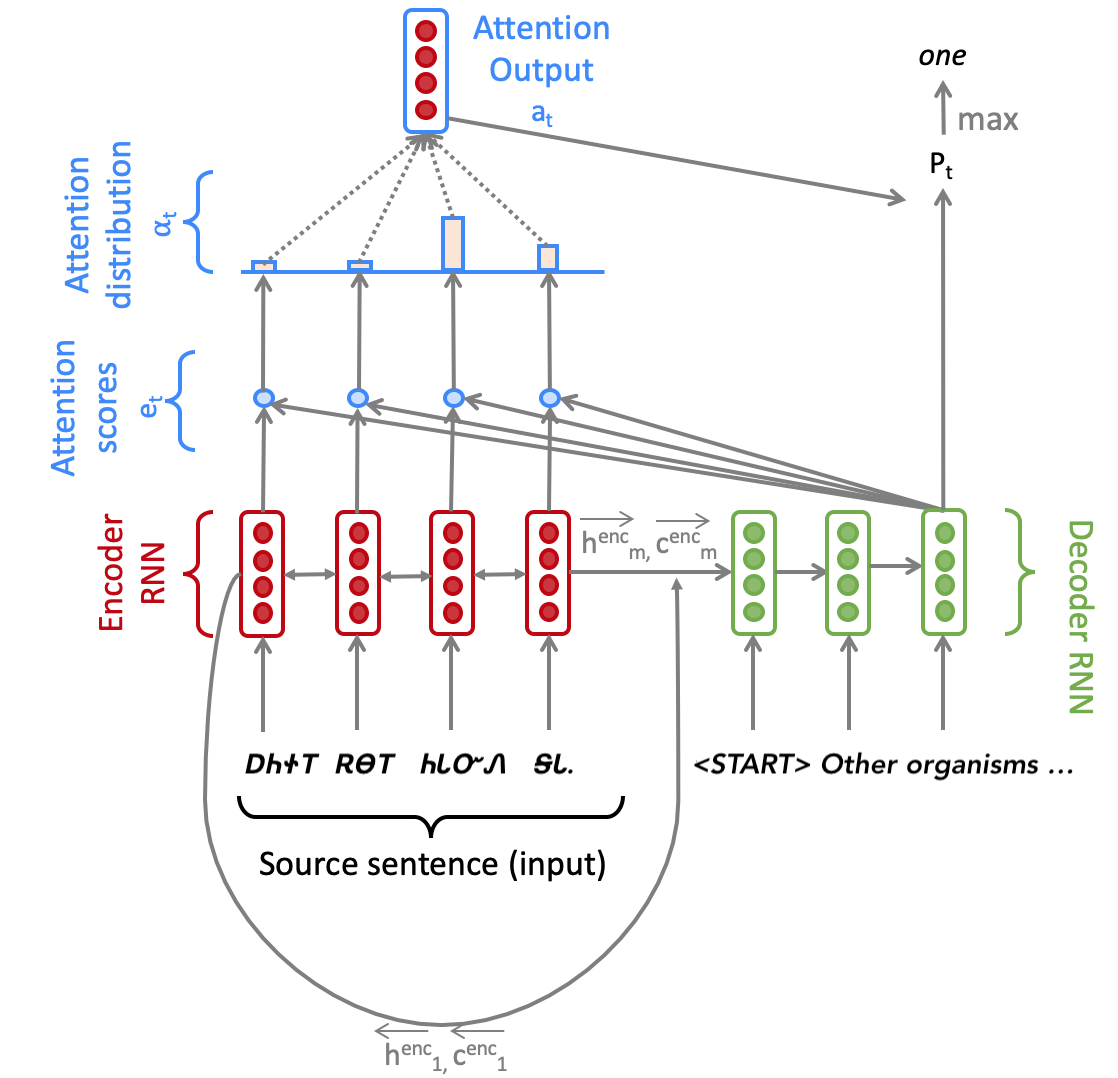
\includegraphics[width=0.7\textwidth]{images/nmt.png}
        \caption{Seq2Seq Model with Multiplicative Attention, shown on the third step of the decoder. Hidden states $\henc_i$ and cell states $\cenc_i$ are defined in the next page.
        }
        \label{nmt-figure}
    \end{center}
\end{figure}

\subsection*{Model description (training procedure)}
Given a sentence in the source language, we look up the subword embeddings from an embeddings matrix, yielding $\bx_1, \dots, \bx_m$ ($\bx_i \in \Real^{e \times 1}$), where $m$ is the length of the source sentence and $e$ is the embedding size. We feed these embeddings to the bidirectional encoder, yielding hidden states and cell states for both the forwards ($\rightarrow$) and backwards ($\leftarrow$) LSTMs. The forwards and backwards versions are concatenated to give hidden states $\henc_i$ and cell states $\cenc_i$:

\begin{align}
    \henc_i = [\hencbw{i}; \hencfw{i}] \enspace &\text{where}\enspace \henc_i \in \Real^{2h \times 1}, \hencbw{i}, \hencfw{i} \in \Real^{h \times 1} &1 \le i \le m \\
    \cenc_i = [\cencbw{i}; \cencfw{i}] \enspace &\text{where} \enspace \cenc_i \in \Real^{2h \times 1}, \cencbw{i}, \cencfw{i} \in \Real^{h \times 1} &1 \le i \le m
\end{align}

We then initialize the decoder's first hidden state $\hdec_0$ and cell state $\cdec_0$ with a linear projection of the encoder's final hidden state and final cell state.\footnote{If it's not obvious, think about why we regard $[\hencbw{1}, \hencfw{m}]$ as the `final hidden state' of the Encoder.}

\begin{align}
    \hdec_0 = \bW_{h}[\hencbw{1}; \hencfw{m}] \enspace &\text{where} \enspace \hdec_0 \in \Real^{h \times 1}, \bW_{h} \in \Real^{h \times 2h}\\
    \cdec_0 = \bW_{c}[\cencbw{1}; \cencfw{m}] \enspace &\text{where} \enspace \cdec_0 \in \Real^{h \times 1}, \bW_{c} \in \Real^{h \times 2h}
\end{align}

With the decoder initialized, we must now feed it a target sentence. On the $t^{th}$ step, we look up the embedding for the $t^{th}$ subword,  $\by_t \in \Real^{e \times 1}$. We then concatenate $\by_t$ with the \textit{combined-output vector} $\bo_{t-1} \in \Real^{h \times 1}$ from the previous timestep (we will explain what this is later down this page!\@) to produce $\overline{\by_t} \in \Real^{(e+h) \times 1}$. Note that for the first target subword (i.e. the start token) $\bo_{0}$ is a zero-vector. We then feed $\overline{\by_t}$ as input to the decoder.

\begin{align}
    \hdec_t, \cdec_t = \text{Decoder}(\overline{\by_t}, \hdec_{t-1}, \cdec_{t-1}) \enspace &\text{where} \enspace \hdec_t \in \Real^{h \times 1}, \cdec_t \in \Real^{h \times 1}\\
\end{align}

We then use $\hdec_t$ to compute multiplicative attention over $\henc_1, \dots, \henc_m$:

\begin{align}
    \be_{t, i} = (\hdec_t)^T\bW_{\text{attProj}}\henc_i \enspace &\text{where} \enspace \be_{t} \in \Real^{m \times 1}, \bW_{\text{attProj}}\in \Real^{h \times 2h} & 1 \le i \le m \\
    \alpha_t= \text{softmax}(\be_t) \enspace &\text{where} \enspace \alpha_t \in \Real^{m \times 1}\\
    \ba_t = \sum_{i=1}^{m}\alpha_{t,i}\henc_i \enspace &\text{where} \enspace \ba_t \in \Real^{2h \times 1}
\end{align}

$\be_{t, i}$ is a scalar, the $i$th element of $\be_{t} \in \Real^{m \times 1}$, computed using the hidden state of the decoder at the $t$th step, $\hdec_t \in \Real^{h \times 1}$, the attention projection $\bW_{\text{attProj}} \in \Real^{h \times 2h}$, and the hidden state of the encoder at the $i$th step, $\henc_i \in \Real^{2h \times 1}$.

We now concatenate the attention output $\ba_t$ with the decoder hidden state $\hdec_t$ and pass this through a linear layer, tanh, and dropout to attain the \textit{combined-output} vector $\bo_{t}$.

\begin{align}
    \bu_{t} = [\ba_{t}; \hdec_t] \enspace &\text{where} \enspace \bu_t \in  \Real^{3h \times 1} \\
    \bv_t = \bW_{u}\bu_t \enspace &\text{where} \enspace \bv_t \in \Real^{h \times 1}, \bW_{u} \in \Real^{h \times 3h}\\
    \bo_t = \text{dropout}(\text{tanh}(\bv_t)) \enspace &\text{where} \enspace \bo_t \in \Real^{h \times 1}
\end{align}

Then, we produce a probability distribution $\bP_t$ over target subwords at the $t^{th}$ timestep:

\begin{align}
    \bP_t = \text{softmax}(\bW_{\text{vocab}}\bo_{t}) \enspace &\text{where} \enspace \bP_t \in \Real^{V_{t} \times 1}, \bW_{\text{vocab}} \in \Real^{V_{t} \times h}
\end{align}

Here, $V_{t}$ is the size of the target vocabulary. Finally, to train the network we then compute the cross entropy loss between $\bP_t$ and $\bg_{t}$, where $\bg_{t}$ is the one-hot vector of the target subword at timestep $t$:

\begin{align}
    J_t(\theta) = \mathrm{CrossEntropy}(\bP_t,\bg_{t})
\end{align}

Here, $\theta$ represents all the parameters of the model and $J_t(\theta)$ is the loss on step $t$ of the decoder.
Now that we have described the model, let's try implementing it for Cherokee to English translation!

\subsection*{Setting up your Virtual Machine}
Follow the instructions in the \href{https://docs.google.com/document/d/10rhknu-xJJCHUQx3DPqKuHT35EqftmZ1rEdR1nJoBFo/edit#heading=h.4tqnggp12z76}{CS224n Azure Guide} (link also provided on website and Ed) in order to create your VM instance. This should take you approximately 45 minutes. Though you will need the GPU to train your model, we strongly advise that you first develop the code locally and ensure that it runs, before attempting to train it on your VM. GPU time is expensive and limited. It takes approximately \textbf{30 minutes to 1 hour} to train the NMT system. We don't want you to accidentally use all your GPU time for debugging your model rather than training and evaluating it. Finally, \textbf{make sure that your VM is turned off whenever you are not using it.}

\textbf{\textcolor{red}{If your Azure subscription runs out of money, your VM will be temporarily locked and inaccessible. If that happens, please fill out a request form \href{https://forms.gle/foFi9p5sQW4wNUTq6}{here}.}}

In order to run the model code on your \textbf{local} machine, please run the following command to create the proper virtual environment:

\begin{lstlisting}
    conda env create --file local_env.yml
\end{lstlisting}

Note that this virtual environment \textbf{will not} be needed on the VM.\newline

\subsection*{Implementation and written questions}

\begin{parts}
    \part [2] (coding) In order to apply tensor operations, we must ensure that the sentences in a given batch are of the same length. Thus, we must identify the longest sentence in a batch and pad others to be the same length. Implement the \texttt{pad\_sents} function in \texttt{utils.py}, which shall produce these padded sentences.

    \part[3] (coding) Implement the \texttt{\_\_init\_\_} function in \texttt{model\_embeddings.py} to initialize the necessary source and target embeddings.

    \part[4] (coding) Implement the \texttt{\_\_init\_\_} function in \texttt{nmt\_model.py} to initialize the necessary model embeddings (using the \texttt{ModelEmbeddings} class from \texttt{model\_embeddings.py}) and layers (LSTM, projection, and dropout) for the NMT system.

    \part[8] (coding) Implement the \texttt{encode} function in \texttt{nmt\_model.py}. This function converts the padded source sentences into the tensor $\bX$, generates $\henc_1, \dots, \henc_m$, and computes the initial state $\hdec_0$ and initial cell $\cdec_0$ for the Decoder. You can run a non-comprehensive sanity check by executing:

    \begin{lstlisting}
    python sanity_check.py 1d
    \end{lstlisting}

    \part[8] (coding) Implement the \texttt{decode} function in \texttt{nmt\_model.py}. This function constructs $\bar{\by}$ and runs the \texttt{step} function over every timestep for the input. You can run a non-comprehensive sanity check by executing:


    \begin{lstlisting}
    python sanity_check.py 1e
    \end{lstlisting}

    \part[10] (coding) Implement the \texttt{step} function in \texttt{nmt\_model.py}. This function applies the Decoder's LSTM cell for a single timestep, computing the encoding of the target subword $\hdec_t$, the attention scores $\be_t$, attention distribution $\alpha_t$, the attention output $\ba_{t}$, and finally the combined output $\bo_t$. You can run a non-comprehensive sanity check by executing:


    \begin{lstlisting}
    python sanity_check.py 1f
    \end{lstlisting}


    \part [3] (written) The \texttt{generate\_sent\_masks()} function in \texttt{nmt\_model.py} produces a tensor called \texttt{enc\_masks}. It has shape (batch size, max source sentence length) and contains 1s in positions corresponding to `pad' tokens in the input, and 0s for non-pad tokens. Look at how the masks are used during the attention computation in the \texttt{step()} function (lines 295-296).

    First explain (in around three sentences) what effect the masks have on the entire attention computation.
    Then explain (in one or two sentences) why it is necessary to use the masks in this way.
\end{parts}

Now it's time to get things running! Execute the following to generate the necessary vocab file:

\begin{lstlisting}
    sh run.sh vocab
\end{lstlisting}

Or if you are on Windows, use the following command instead. Make sure you execute this in an environment that has python in path. For example, you can run this in the terminal of your IDE or your Anaconda prompt.


\begin{lstlisting}
    run.bat vocab
\end{lstlisting}

As noted earlier, we recommend that you develop the code on your personal computer. Confirm that you are running in the proper conda environment and then execute the following command to train the model on your local machine:

\begin{lstlisting}
    sh run.sh train_local
    (Windows) run.bat train_local
\end{lstlisting}

To help with monitoring and debugging, the starter code uses tensorboard to log loss and perplexity during training using TensorBoard\footnote{https://pytorch.org/docs/stable/tensorboard.html}. TensorBoard provides tools for logging and visualizing training information from experiments. To open TensorBoard, run the following in your conda environment:

\begin{lstlisting}
   tensorboard --logdir=runs
\end{lstlisting}

You should see a significant decrease in loss during the initial iterations. Once you have ensured that your code does not crash (i.e. let it run till \texttt{iter 10} or \texttt{iter 20}), power on your VM from the Azure Web Portal. Then read the \textit{Managing Code Deployment to a VM} section of our \href{https://docs.google.com/document/d/1jtANWXbIYXMZO_2X7jupauPxcEbz-TVJkdatg4gzOdk}{Practical Guide to VMs} (link also given on website and Ed) for instructions on how to upload your code to the VM.

Next, install necessary packages to your VM by running:

\begin{lstlisting}
    pip install -r gpu_requirements.txt
\end{lstlisting}

Finally, turn to the \textit{Managing Processes on a VM} section of the Practical Guide and follow the instructions to create a new tmux session. Concretely, run the following command to create tmux session called \texttt{nmt}.
\begin{lstlisting}
    tmux new -s nmt
\end{lstlisting}


Once your VM is configured and you are in a tmux session, execute:
\begin{lstlisting}
    sh run.sh train
    (Windows) run.bat train
\end{lstlisting}

Once you know your code is running properly, you can detach from session and close your ssh connection to the server. To detach from the session, run:
\begin{lstlisting}
    tmux detach
\end{lstlisting}

You can return to your training model by ssh-ing back into the server and attaching to the tmux session by running:

\begin{lstlisting}
    tmux a -t nmt
\end{lstlisting}

\begin{parts}
    \setcounter{partno}{7}
    \part[3] (written) Once your model is done training (\textbf{this should take under 1 hour on the VM}), execute the following command to test the model:
    \begin{lstlisting}
sh run.sh test
(Windows) run.bat test
    \end{lstlisting}
    Please report the model's corpus BLEU Score. It should be larger than 10.

    \part[4] (written) In class, we learned about dot product attention, multiplicative attention, and additive attention. As a reminder, dot product attention is $\be_{t,i} = \bs_t^T\bh_i$, multiplicative attention is $\be_{t,i} = \bs_t^T\bW\bh_i$, and additive attention is $\be_{t,i} = \bv^T \text{tanh}(\bW_1\bh_i + \bW_2\bs_t)$.

    \ifans{
        Corpus BLEU: 13.110528453394458
    } \fi \newline

    \begin{subparts}
        \subpart[2] Explain one advantage and one disadvantage of \textit{dot product attention} compared to multiplicative attention.
        \subpart[2] Explain one advantage and one disadvantage of \textit{additive attention} compared to multiplicative attention.
    \end{subparts}
\end{parts}

        \newpage
        \usepackage{hyperref}\graphicspath{ {images/} }

\titledquestion{Analyzing NMT Systems}[33]

\begin{parts}
    \part[3] In part 1, we modeled our NMT problem at a subword-level. That is, given a sentence in the source language, we looked up subword components from an embeddings matrix. Alternatively, we could have modeled the NMT problem at the word-level, by looking up whole words from the embeddings matrix. Why might it be important to model our Cherokee-to-English NMT problem at the subword-level vs. the whole word-level? (Hint: Cherokee is a polysynthetic language.) \\
    \ifans{
        Since Cherokee is a polysynthetic language, it may have a very large vocabulary and a large embedding matrix
        may be needed to implement effective word-level NMT models, which is impractical. Also, subword models may capture
        morphosyntactic relations for polysynthetic languages more effectively.
    } \fi \\

    \part[3] Transliteration is the representation of letters or words in the characters of another alphabet or script based on phonetic similarity. For example, the transliteration of {\cherokeefam Ꮳ⁠Ꮕ⁠Ꮤ⁠Ꮝ⁠Ꭺ} (which translates to "do you know") from Cherokee letters to Latin script is tsanvtasgo. In the Cherokee language, "ts-" is a common prefix in many words, but the Cherokee character {\cherokeefam Ꮳ} is "tsa". Using this example, explain why when modeling our Cherokee-to-English NMT problem at the subword-level, training on transliterated Cherokee text may improve performance over training on original Cherokee characters.(Hint: A prefix is a morpheme.) \\
    \ifans{
        Training on transliterated Cherokee text could make it easier to separate words into morphemes, because the original
        Cherokee characters may contain inseparable combinations of morphemes.
    } \fi \\

    \part[3] One challenge of training successful NMT models is lack of language data, particularly for resource-scarce languages like Cherokee. One way of addressing this challenge is with multilingual training, where we train our NMT on multiple languages (including Cherokee). You can read more about multilingual training here:\newline \url{https://ai.googleblog.com/2019/10/exploring-massively-multilingual.html}.\newline How does multilingual training help in improving NMT performance with low-resource languages?\\
    \ifans{
        Multilingual model can somehow transfer parameters from relatively high-resource languages and improve NMT performance
        with low-resource languages.
    } \fi \\

    \part[6] Here we present a series of errors we found in the outputs of our NMT model (which is the same as the one you just trained). For each example of a reference (i.e., `gold') English translation, and NMT (i.e., `model') English translation, please:

    \begin{enumerate}
        \item Identify the error in the NMT translation.
        \item Provide possible reason(s) why the model may have made the error (either due to a specific linguistic construct or a specific model limitation).
        \item Describe one possible way we might alter the NMT system to fix the observed error. There are more than one possible fixes for an error. For example, it could be tweaking the size of the hidden layers or changing the attention mechanism.
    \end{enumerate}

    Below are the translations that you should analyze as described above. Only analyze the underlined error in each sentence. Rest assured that you don't need to know Cherokee to answer these questions. You just need to know English! If, however, you would like additional color on the source sentences, feel free to use a resource like \url{https://www.cherokeedictionary.net/} to look up words.

    \begin{subparts}
        \subpart[2]
        \textbf{Source Sentence:} \textit{{\cherokeefam ᏄᏩᏁᎰᎾ ᏕᎪᏣᎳᎩᏍᎬ, ᎯᎠ ᏄᏍᏕ ᏚᏏᎳᏛ: ᏧᏓᎴᏅᏓ ᏕᎪᏒᏍᎦ ᏧᏏᎳᏛᏙᏗ ᎠᏍᏓ ᎧᏅᏂᏍᎩ.        }}\newline
        \textbf{Reference Translation:} \textit{When \underline{she} was finished ripping things out, \underline{her} web looked something like this: }\newline
        \textbf{NMT Translation:} \textit{When \underline{it} was gone out of the web, \underline{he} said the web in the web.} \\
        \ifans{
            The NMT model uses "it" and "he" to refer to the same object. It seems that the NMT model has not really learned the
            target language grammar. To fix this, run more epoches, add more training data, and increase the size of the hidden layers may help.
        } \fi \\

        \subpart[2]
        \textbf{Source Translation}: \textit{{\cherokeefam ᎤᏍᏗ ᎢᏈᎬᎢ, ᎦᏙᏊᎢ? ᎤᏓᏛᏛᏁᎢ ᎤᏍᏗ ᎠᏧᏣ.}}\newline
        \textbf{Reference Translation}: \textit{What's wrong \underline{little} tree? the boy asked.}\newline
        \textbf{NMT Translation}: \textit{ The \underline{little little little little little} tree? asked him.} \\
        \ifans{
            The NMT Translation repeated the word "little" for 5 times. It is possible that the model attends to the same parts
            of the source sentence and calculated a similar probability distribution. It may help to implement self-attention
            mechanism for the NMT model.
        } \fi \\

        \subpart[2]
        \textbf{Source Sentence:} \textit{{\cherokeefam “ᎤᏓᎸᏉᏗ ᏂᎨᏒᎾ,” ᎤᏛᏁ ᎰᎻ.}}\newline
        \textbf{Reference Translation:} \textit{\underline{“ ‘Humble,’ ”} said Mr. Zuckerman}\newline
        \textbf{NMT Translation:} \textit{\underline{“It’s not a lot,”} said Mr. Zuckerman.}\\
        \ifans{
            The model used "it's not a lot" to express the meaning of "humble." It is possible that the training data of the target
            language does not contain the word "humble." To fix the problem, add more training data to the model or apply a character-based/hybrid NMT model
            in this situation.
        } \fi \\
    \end{subparts}

    \part[4] Now it is time to explore the outputs of the model that you have trained! The test-set translations your model produced in question \texttt{1-i} should be located in \texttt{outputs/test\_outputs.txt}.
    \begin{subparts}
        \subpart[2] Find a line where the predicted translation is correct for a long (4 or 5 word) sequence of words. Check the training target file (English); does the training file contain that string (almost) verbatim? If so or if not, what does this say about what the MT system learned to do? \\
        \ifans{
            Correct sequence of words: \textit{I want to see a little tree, and the frog}. \\
            The string \textit{I want to see} found verbatim in the training data. This indicates that the MT system somehow
            built a language model based on the target training data.

        } \fi \\

        \subpart[2] Find a line where the predicted translation starts off correct for a long (4 or 5 word) sequence of words, but then diverges (where the latter part of the sentence seems totally unrelated). What does this say about the model's decoding behavior? \\
        \ifans{\\
        \textit{It was tired of it, it was tired of the day, and in the day of the day he had tired of the morning.} \\
        It seems that the decoder is not aware of what it said a few time-steps ago.

        } \fi \\
    \end{subparts}

    \part[14] BLEU score is the most commonly used automatic evaluation metric for NMT systems. It is usually calculated across the entire test set, but here we will consider BLEU defined for a single example.\footnote{This definition of sentence-level BLEU score matches the \texttt{sentence\_bleu()} function in the \texttt{nltk} Python package. Note that the NLTK function is sensitive to capitalization. In this question, all text is lowercased, so capitalization is irrelevant. \\ \url{http://www.nltk.org/api/nltk.translate.html\#nltk.translate.bleu_score.sentence_bleu}
    }
    Suppose we have a source sentence $\bs$, a set of $k$ reference translations $\br_1,\dots,\br_k$, and a candidate translation $\bc$. To compute the BLEU score of $\bc$, we first compute the \textit{modified $n$-gram precision} $p_n$ of $\bc$, for each of $n=1,2,3,4$, where $n$ is the $n$ in \href{https://en.wikipedia.org/wiki/N-gram}{n-gram}:
    \begin{align}
        p_n = \frac{ \displaystyle \sum_{\text{ngram} \in \bc} \min \bigg( \max_{i=1,\dots,k} \text{Count}_{\br_i}(\text{ngram}), \enspace \text{Count}_{\bc}(\text{ngram}) \bigg) }{\displaystyle \sum_{\text{ngram}\in \bc} \text{Count}_{\bc}(\text{ngram})}
    \end{align}
    Here, for each of the $n$-grams that appear in the candidate translation $\bc$, we count the maximum number of times it appears in any one reference translation, capped by the number of times it appears in $\bc$ (this is the numerator). We divide this by the number of $n$-grams in $\bc$ (denominator). \newline

    Next, we compute the \textit{brevity penalty} BP. Let $len(c)$ be the length of $\bc$ and let $len(r)$ be the length of the reference translation that is closest to $len(c)$ (in the case of two equally-close reference translation lengths, choose $len(r)$ as the shorter one).
    \begin{align}
        BP =
        \begin{cases}
            1 & \text{if } len(c) \ge len(r) \\
            \exp \big( 1 - \frac{len(r)}{len(c)} \big) & \text{otherwise}
        \end{cases}
    \end{align}
    Lastly, the BLEU score for candidate $\bc$ with respect to $\br_1,\dots,\br_k$ is:
    \begin{align}
        BLEU = BP \times \exp \Big( \sum_{n=1}^4 \lambda_n \log p_n \Big)
    \end{align}
    where $\lambda_1,\lambda_2,\lambda_3,\lambda_4$ are weights that sum to 1. The $\log$ here is natural log.
    \newline
    \begin{subparts}
        \subpart[5] Please consider this example\footnote{Due to data availability, many Cherokee sentences with English reference translations are from the Bible. This example is John 1:5. The two reference translations are from the New International Version and the New King James Version translations of the Bible.}: \newline
        Source Sentence $\bs$: \textbf{{\cherokeefam ᎠᎴ ᎾᏍᎩ ᎢᎦ-ᎦᏘᏍᏗᏍᎩ ᎤᎵᏏᎬ ᏚᎸᏌᏕᎢ ᎤᎵᏏᎩᏃ ᎥᏝ ᏱᏚᏓᏂᎸᏤᎢ}}
        \newline
        Reference Translation $\br_1$: \textit{the light shines in the darkness and the darkness has not overcome it}
        \newline
        Reference Translation $\br_2$: \textit{and the light shines in the darkness and the darkness did not comprehend it}

        NMT Translation $\bc_1$: and the light shines in the darkness and the darkness can not comprehend

        NMT Translation $\bc_2$: the light shines the darkness has not in the darkness and the trials

        Please compute the BLEU scores for $\bc_1$ and $\bc_2$. Let $\lambda_i=0.5$ for $i\in\{1,2\}$ and $\lambda_i=0$ for $i\in\{3,4\}$ (\textbf{this means we ignore 3-grams and 4-grams}, i.e., don't compute $p_3$ or $p_4$). When computing BLEU scores, show your working (i.e., show your computed values for $p_1$, $p_2$, $len(c)$, $len(r)$ and $BP$). Note that the BLEU scores can be expressed between 0 and 1 or between 0 and 100. The code is using the 0 to 100 scale while in this question we are using the \textbf{0 to 1} scale.
        \newline

        Which of the two NMT translations is considered the better translation according to the BLEU Score? Do you agree that it is the better translation?\\
        \ifans{ \\
        For $\bc_1$, $p_1 = \frac{12}{13} $, $p_2 = \frac{10}{12}$, $len(c) = 13$, $len(r) = 13$, $BP=1$,\\ $BLEU = BP \times \exp(0.5\log{p_1}+0.5\log{p_2}) = 0.8770580193070293$.\\~\\
        For $\bc_2$, $p_1 = \frac{11}{13} $, $p_2 = \frac{9}{12}$, $len(c) = 13$, $len(r) = 13$, $BP=1$,\\ $BLEU = BP \times \exp(0.5\log{p_1}+0.5\log{p_2}) = 0.7966275068156915$.\\~\\
        According to the BLEU Score, $\bc_1$ is considered the better translation. I agree that it is the better translation.
        } \fi \\

        \subpart[5] Our hard drive was corrupted and we lost Reference Translation $\br_2$. Please recompute BLEU scores for $\bc_1$ and $\bc_2$, this time with respect to $\br_1$ only. Which of the two NMT translations now receives the higher BLEU score? Do you agree that it is the better translation?\\
        \ifans{\\
        For $\bc_1$, $p_1 = \frac{10}{13} $, $p_2 = \frac{8}{12}$, $len(c) = 13$, $len(r) = 13$, $BP=1$,\\ $BLEU = BP \times \exp(0.5\log{p_1}+0.5\log{p_2}) = 0.7161148740394329$.\\~\\
        For $\bc_2$, $p_1 = \frac{11}{13} $, $p_2 = \frac{9}{12}$, $len(c) = 13$, $len(r) = 13$, $BP=1$,\\ $BLEU = BP \times \exp(0.5\log{p_1}+0.5\log{p_2}) = 0.7966275068156915$.\\~\\
        According to the BLEU Score, $\bc_2$ is considered the better translation. I don't agree that it is the better translation because it is confusing and contains some syntactic errors.
        } \fi \\

        \subpart[2] Due to data availability, NMT systems are often evaluated with respect to only a single reference translation. Please explain (in a few sentences) why this may be problematic. In your explanation, discuss how the BLEU score metric assesses the quality of NMT translations when there are multiple reference transitions versus a single reference translation.\\
        \ifans{
            When a candidate translation is compared to a single reference translation, the representation of the relevant n-grams
            that should be matched to obtain a high BLEU Score is noisy.
            Therefore, the BLEU score for an appropriate translation may also be relatively low.
            When there are multiple reference translations, the NMT system gets more flexibility to interpret and decode the source
            sentence and is more likely to get a fair BLEU Score.
        } \fi \\
        \subpart[2] List two advantages and two disadvantages of BLEU, compared to human evaluation, as an evaluation metric for Machine Translation.\\
        \ifans{\\
        \textbf{Advantages}
            \begin{itemize}
                \item BLEU makes NMT evaluation fast, economical.
                \item It is language independent and easy to understand.
            \end{itemize}
            \textbf{Disadvantages}
            \begin{itemize}
                \item Its true quality remains far below human translations.
                \item It does not really consider semantics or sentence structures.
            \end{itemize}
        } \fi \\
    \end{subparts}
\end{parts}

    \end{questions}

    \Large{\textbf{Submission Instructions}}

\normalsize
You shall submit this assignment on GradeScope as two submissions -- one for ``Assignment 4 [coding]" and another for `Assignment 4 [written]":
\begin{enumerate}
    \item Run the \texttt{collect\_submission.sh} script on Azure to produce your \texttt{assignment4.zip} file. You can use \href{http://www.hypexr.org/linux_scp_help.php}{scp} to transfer files between Azure and your local computer.
    \item Upload your \texttt{assignment4.zip} file to GradeScope to ``Assignment 4 [coding]".
    \item Upload your written solutions to GradeScope to ``Assignment 4 [written]". When you submit your assignment, make sure to tag all the pages for each problem according to Gradescope's submission directions. Points will be deducted if the submission is not correctly tagged.
\end{enumerate}
\end{document}